\documentclass[conference]{IEEEtran}
\usepackage{cite}
% cite.sty was written by Donald Arseneau
% V1.6 and later of IEEEtran pre-defines the format of the cite.sty package
% \cite{} output to follow that of the IEEE. Loading the cite package will
% result in citation numbers being automatically sorted and properly
% "compressed/ranged". e.g., [1], [9], [2], [7], [5], [6] without using
% cite.sty will become [1], [2], [5]--[7], [9] using cite.sty. cite.sty's
% \cite will automatically add leading space, if needed. Use cite.sty's
% noadjust option (cite.sty V3.8 and later) if you want to turn this off
% such as if a citation ever needs to be enclosed in parenthesis.
% cite.sty is already installed on most LaTeX systems. Be sure and use
% version 5.0 (2009-03-20) and later if using hyperref.sty.
% The latest version can be obtained at:
% http://www.ctan.org/pkg/cite
% The documentation is contained in the cite.sty file itself.


\usepackage{algorithmic}
% algorithmic.sty was written by Peter Williams and Rogerio Brito.
% This package provides an algorithmic environment fo describing algorithms.
% You can use the algorithmic environment in-text or within a figure
% environment to provide for a floating algorithm. Do NOT use the algorithm
% floating environment provided by algorithm.sty (by the same authors) or
% algorithm2e.sty (by Christophe Fiorio) as the IEEE does not use dedicated
% algorithm float types and packages that provide these will not provide
% correct IEEE style captions. The latest version and documentation of
% algorithmic.sty can be obtained at:
% http://www.ctan.org/pkg/algorithms
% Also of interest may be the (relatively newer and more customizable)
% algorithmicx.sty package by Szasz Janos:
% http://www.ctan.org/pkg/algorithmicx




% *** ALIGNMENT PACKAGES ***
%
%\usepackage{array}
% Frank Mittelbach's and David Carlisle's array.sty patches and improves
% the standard LaTeX2e array and tabular environments to provide better
% appearance and additional user controls. As the default LaTeX2e table
% generation code is lacking to the point of almost being broken with
% respect to the quality of the end results, all users are strongly
% advised to use an enhanced (at the very least that provided by array.sty)
% set of table tools. array.sty is already installed on most systems. The
% latest version and documentation can be obtained at:
% http://www.ctan.org/pkg/array


% IEEEtran contains the IEEEeqnarray family of commands that can be used to
% generate multiline equations as well as matrices, tables, etc., of high
% quality.




% *** SUBFIGURE PACKAGES ***
%\ifCLASSOPTIONcompsoc
%  \usepackage[caption=false,font=normalsize,labelfont=sf,textfont=sf]{subfig}
%\else
%  \usepackage[caption=false,font=footnotesize]{subfig}
%\fi
% subfig.sty, written by Steven Douglas Cochran, is the modern replacement
% for subfigure.sty, the latter of which is no longer maintained and is
% incompatible with some LaTeX packages including fixltx2e. However,
% subfig.sty requires and automatically loads Axel Sommerfeldt's caption.sty
% which will override IEEEtran.cls' handling of captions and this will result
% in non-IEEE style figure/table captions. To prevent this problem, be sure
% and invoke subfig.sty's "caption=false" package option (available since
% subfig.sty version 1.3, 2005/06/28) as this is will preserve IEEEtran.cls
% handling of captions.
% Note that the Computer Society format requires a larger sans serif font
% than the serif footnote size font used in traditional IEEE formatting
% and thus the need to invoke different subfig.sty package options depending
% on whether compsoc mode has been enabled.
%
% The latest version and documentation of subfig.sty can be obtained at:
% http://www.ctan.org/pkg/subfig




% *** FLOAT PACKAGES ***
%
%\usepackage{fixltx2e}
% fixltx2e, the successor to the earlier fix2col.sty, was written by
% Frank Mittelbach and David Carlisle. This package corrects a few problems
% in the LaTeX2e kernel, the most notable of which is that in current
% LaTeX2e releases, the ordering of single and double column floats is not
% guaranteed to be preserved. Thus, an unpatched LaTeX2e can allow a
% single column figure to be placed prior to an earlier double column
% figure.
% Be aware that LaTeX2e kernels dated 2015 and later have fixltx2e.sty's
% corrections already built into the system in which case a warning will
% be issued if an attempt is made to load fixltx2e.sty as it is no longer
% needed.
% The latest version and documentation can be found at:
% http://www.ctan.org/pkg/fixltx2e


%\usepackage{stfloats}
% stfloats.sty was written by Sigitas Tolusis. This package gives LaTeX2e
% the ability to do double column floats at the bottom of the page as well
% as the top. (e.g., "\begin{figure*}[!b]" is not normally possible in
% LaTeX2e). It also provides a command:
%\fnbelowfloat
% to enable the placement of footnotes below bottom floats (the standard
% LaTeX2e kernel puts them above bottom floats). This is an invasive package
% which rewrites many portions of the LaTeX2e float routines. It may not work
% with other packages that modify the LaTeX2e float routines. The latest
% version and documentation can be obtained at:
% http://www.ctan.org/pkg/stfloats
% Do not use the stfloats baselinefloat ability as the IEEE does not allow
% \baselineskip to stretch. Authors submitting work to the IEEE should note
% that the IEEE rarely uses double column equations and that authors should try
% to avoid such use. Do not be tempted to use the cuted.sty or midfloat.sty
% packages (also by Sigitas Tolusis) as the IEEE does not format its papers in
% such ways.
% Do not attempt to use stfloats with fixltx2e as they are incompatible.
% Instead, use Morten Hogholm'a dblfloatfix which combines the features
% of both fixltx2e and stfloats:
%
% \usepackage{dblfloatfix}
% The latest version can be found at:
% http://www.ctan.org/pkg/dblfloatfix

\usepackage[acronym]{glossaries}
\usepackage{amsmath}
\usepackage{graphicx}
\usepackage{amsfonts}
\usepackage{mathtools}
\usepackage{amsmath}
\usepackage{amssymb}
\usepackage{hyperref}
\usepackage{float}
\usepackage{caption}
\usepackage{subcaption}
% \usepackage[numbers]{natbib}
\usepackage{cleveref}
\usepackage{bm}
\usepackage{booktabs}

% correct bad hyphenation here
\hyphenation{op-tical net-works semi-conduc-tor}
\renewcommand{\citedash}{--}
\DeclareMathOperator*{\argmin}{arg\,min}
\newcommand{\norm}[1]{\left\lVert#1\right\rVert}

\makeglossaries{}
% Model
\newacronym{mfms}{MFMS}{Multifrequency Multistage Radiolocation System}
% General Definitions
\newacronym{tx}{TX}{Transmission}
\newacronym{rx}{RX}{Receive}
\newacronym{em}{EM}{Electromagnetic}
\newacronym{rf}{RF}{Radio Frequency}
\newacronym{lora}{LoRa}{Long Range Radio}
\newacronym{wifi}{WiFi}{Wireless Fidelity}
\newacronym{bt}{BT}{Bluetooth}
\newacronym{rss}{RSS}{Received Signal Strength}
% Learning Models
\newacronym{rbm}{RBM}{Restricted Boltzman Machine}
\newacronym{fnn}{FNN}{Feedforward Neural Network}
\newacronym{nn}{NN}{Neural Network}
\newacronym{rnn}{RNN}{Recurrent Neural Network}
\newacronym{cnn}{CNN}{Convolutional Neural Network}
\newacronym{lan}{LAN}{Local Area Network}
\newacronym{gru}{GRU}{Gated Recurrent Unit}
\newacronym{rbe}{RBE}{Recursive Bayesian Estimation}
\newacronym{pf}{PF}{Particle Filter}
% Radio Wave Bands
\newacronym{vlf}{VLF}{Very Low Frequency}
\newacronym{lf}{LF}{Low Frequency}
\newacronym{mf}{MF}{Medium Frequency}
\newacronym{hf}{HF}{High Frequency}
\newacronym{vhf}{VHF}{Very High Frequency}
\newacronym{uhf}{UHF}{Ultra High Frequency}
\newacronym{shf}{SHF}{Super High Frequency}
\newacronym{ehf}{EHF}{Extremely High Frequency}
\newacronym{thf}{THF}{Tremendously High Frequency}
% Essential and Propagation Models
\newacronym{ldpl}{LDPL}{Log-distance Path Loss}
\newacronym{ffse}{FFSE}{Friis' Free Space Equation}
\newacronym{pl}{PL}{Path Loss}
\newacronym{ips}{IPS}{Indoor Positioning System}
\newacronym{irl}{IRL}{Indoor Radiolocatining System}
\newacronym{firl}{FIRL}{Fingerprinting-based Indoor Radiolocationing Systems}
\newacronym{fpips}{FPIPS}{Fingerprinting-based Indoor Positioning System}
\newacronym{los}{LOS}{Line-of-sight}
\newacronym{nlos}{N-LOS}{Non-Line-of-sight}
% Institutes
\newacronym{itu}{ITU}{International Telecommunication Union}
\newacronym{ieee}{IEEE}{Institute of Electrical and Electronics Engineers}
\newacronym{fcc}{FCC}{Federal Communications Commision}

\begin{document}
%
% paper title
% Titles are generally capitalized except for words such as a, an, and, as,
% at, but, by, for, in, nor, of, on, or, the, to and up, which are usually
% not capitalized unless they are the first or last word of the title.
% Linebreaks \\ can be used within to get better formatting as desired.
% Do not put math or special symbols in the title.
\title{A Multifrequency Multistage Fingerprinting-based Radiolocation System}


% author names and affiliations
% use a multiple column layout for up to three different
% affiliations
\author{\IEEEauthorblockN{Murat Ambarkutuk}
\IEEEauthorblockA{
Mechanical Engineering Department, \\
Virginia Polytechnic Institute and State University, \\
Blacksburg, Virginia, USA
Email:murata@vt.edu
}\and
\IEEEauthorblockN{Tomonari Furukawa}
\IEEEauthorblockA{
Mechanical Engineering Department, \\
Virginia Polytechnic Institute and State University, \\
Blacksburg, Virginia, USA
Email: tomonari@vt.edu
}}

\maketitle

% As a general rule, do not put math, special symbols or citations
% in the abstract
\begin{abstract}
    This paper presents a multifrequency and multistage indoor fingerprinting-based radiolocation system.
    The proposed system relies on a 900 MHz and with 2.4 GHz radios based on 802.15.4 protocol.
    By exploiting different propagation characteristics of different \gls{rf} signal wave within a \gls{gru} framework, \gls{rss} and \gls{rtt} measurements are used for indoor localization purposes.
    % where a Deep Learning framework utilized to fully exploit the information from signal maps of various Access Points (AP) available in an environment.
    Similar to conventional fingerprinting systems, the system is consisted of two phases: data acquisition and learning (offline), and localization (online).
    In offline phase, the propagation function for each \gls{an} and path loss exponent is learned by a recurrent network consisted of \gls{gru} from \gls{rss} and \gls{rtt} measurements, whereas the online phase contains different stages of localization and an information fusion stage.
    \textit{Add some result once get it}
\end{abstract}

% For peer review papers, you can put extra information on the cover
% page as needed:
% \ifCLASSOPTIONpeerreview
% \begin{center} \bfseries EDICS Category: 3-BBND \end{center}
% \fi
%
% For peerreview papers, this IEEEtran command inserts a page break and
% creates the second title. It will be ignored for other modes.
\IEEEpeerreviewmaketitle{}
\glsresetall{}

\section{Introduction}
  % The radio waves ..
  % Since \gls{rf} has become ubiquitious, it started being utilized in different applications varying from customer tracking indoors to robot localization. % more varying examples would be good.
  % However it is available, the information can be extracted from is prone to (suffers from) being sparse and severely effected by infrasracture of environments where WiFi based systems are deployed.
  % Amongst all the applications that WiFi signal can be used, robot localization is a problem where it is required to have higher level of success in localization accuracy and shorter localization time.
  % \textit{The main contributions of this paper is that the proposed technique can handle sparse, noisy RSS measurements acquired from the off-the-shelf AP's under LoS and NLoS situations, while achieving comparable localization accuracy to thes state-of-the-art methods.}
  %
  % The success of the systems relying on the WiFi signal, in general, suffers from the phenomenon called Multipath Effect in which the AP is not in the direct line of sight and the EM waves from the AP where the received signal is propagated through non-line-of-sight, i.e.~concrete and glass walls.
  % Although there is some effort to either model or estimate the Multipath Effect to componsate its effects on the systems~\cite{cai2015identification}, it is still an open problem in the field in order to achieve the same level of success under NLoS observations.
  % %One way to componsate the multipath effect is to find out the first the time epoch the signal is acquired; however, some of these operations require significant change in hardware so that  \# \#.
  % \textit{The proposed system can inherently handle multipath effect, since machine not only can reduce complexity of overall design of the system but also can capture deeper information from the radio maps.}
  % % \textit{More explanation regarding the multipath effect is needed here to emphasize that machine learning algorithms can inherently handle it.}
  %
  % Another problem with the WiFi signal which makes it difficult to employ it as the main information source is that the signal acquired is not reliable.
  % Figure~\ref{fig-variance} shows the acquired RSS information acquired with stationary client from the AP's both line-of-sight and non-line-of-sight positions in time.
  % The figure clearly depicts that even for stationary clients, the RSSI readings greatly deviates from the mean in time.
  % % \#\textit{gotta mention that deviation makes it not reliable}.
  % To be able to extract relatively reliable information, some hardware and software changes proposed to incorporate Channel State Information (CSI) provided by Orthogonal Frequency-Division Multiplexing (OFDM) forming WiFi protocol.
  % As~\cite{gao2015channel} suggests/proves, the CSI information provides significantly reliable information.
  % However, to be able to acquire CSI information, a specific type of NIC should be used with a specific type of firmware.
  % This makes it hard to deploy proposed system on Embedded-devices, IoT's and robotic systems.\textit{, while the proposed system can be deployed to almost-any arbitrary system thanks to the simplicity of the design.}
  %
  % % \textit{Nail the idea Machine Learning stuff can be deployed practically everywhere}
  %
  % The paper is organized as follows.
  % The following section reviews the literature regarding robot localization with WiFi signal.
  % In Sec.~\ref{sec-PF}, we formalize the problem.
  % Section~\ref{sec-SD} thoroughly explains the proposed system.
  % The experimentation and the results are  in Sec.~\ref{sec-EX}.
  % We outline our observation and conclusions in the final section.

\begin{figure*}[!pht]
  \centering
  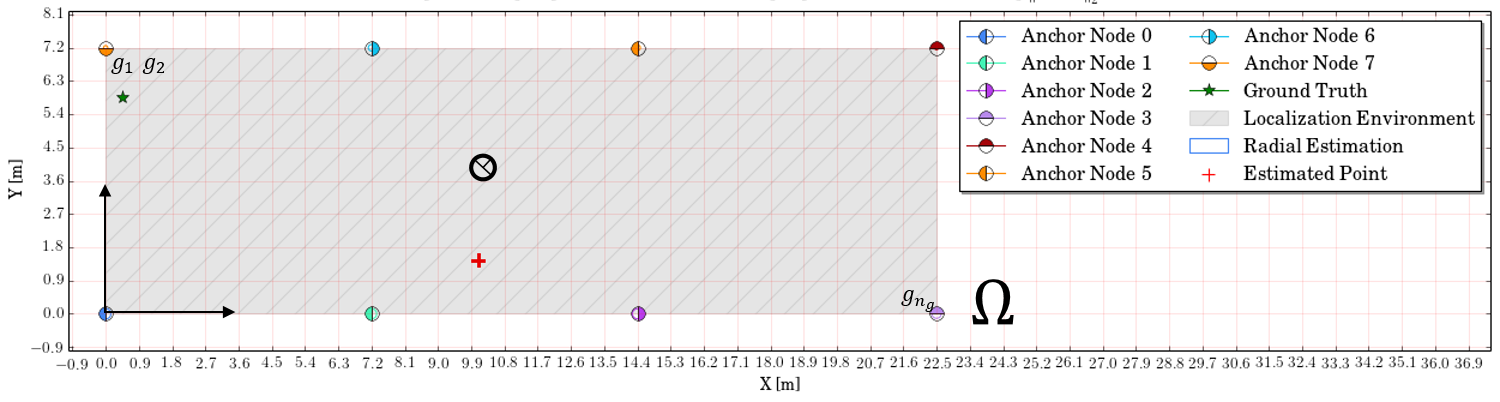
\includegraphics[width=\linewidth]{figures/omega.png}
  \caption{\label{fig:omega} Localization Environment}
\end{figure*}

\section{Fundamentals of Radio Wave Propagation in Radiolocationing}
\label{sec:fundamentals}
    This section will cover the fundamentals of radio wave propagation in regards to \gls{firl}.
    \Gls{firl}s are consisted of two main phases.
    The first phase, i.e.\ offline phase,  involves with collecting some form of measurements about the anchor nodes placed in the environment, with corresponding positions.
    Let $m^i_j$ and $d^i_j$ to be the measurement obtained from anchor node $i$ at a location $j$, and the radial distance of between location $j$ and the anchor node $i$, respectively.
    The measurement space $\bm{m}^i=\{m^i_j | i=1 \ldots n_{node}, j=1 \ldots n_{loc}\}$ are often constructed in either frequency domain [refer CSI], or time domain.
    % The collected measurements are used to approximate the propagation function for each anchor node.
    The measurements are then used to approximate the propagation function $f^i_d$ of each anchor node.

    \begin{equation}
        f^i_d: \bm{m}^i \mapsto \bm{d}^i
    \end{equation}

    One of the most popular fingerprint is \gls{rss} in \gls{firl}s due to its simplicity in acquiring the fingerprints.
    The fundamental relationship between transmitted and received signal strengths $P_t$ and $P_r(d)$ occurred between ideal antennas in an empty space with a distance $d$ separation is characterized by \gls{ffse} given below~\cite{friis1946note}.

    \begin{equation}
        \label{eq:friisWatts}
            P_r(d) = \dfrac{P_t  G_t  G_r \lambda^2}{{\left(4 \pi d\right)}^2}
    \end{equation}

    % In \Cref{eq:friisWatts}, $P_r(d)$ and $P_t$ denote received, and transmitted signal strengths with $d$ meters separation between two antennas in Watts, respectively.
    In \Cref{eq:friisWatts}, $G_t$, and $G_r$ denote unitless gains of transmitter and receiver antennas, respectively, whereas $\lambda$ is the wavelength of the radio wave.
    However well-known, \gls{ffse} is not able to model propagation mechanisms, i.e.\ reflection, diffraction or scattering occurring along the the propagation path, due to the fact that it can only model \gls{los} propagation.
    Thus, it is often impractical to utilize it in indoor localization problems where reflection and diffraction occurs along the propagation path.
    Moreover, since the received signal strength is often minuscule level, \gls{ffse} is denoted in decibel scale relative to a milliwatt.

    \begin{equation}
      \begin{split}
        \label{eq:friisdBm}
        \widetilde{P}_r(d) &= \widetilde{P}_t + 10 \log{G_t} + 10 \log{G_r} + \\
        & 20 \log{\lambda} - 20 \log{d} - 20 \log{4 \pi}
      \end{split}
    \end{equation}
    $\widetilde{P}_r(d)$ and $\widetilde{P}_t$ represent received and transmitted signal strengths decibel scale.
    However, neither \Cref{eq:friisWatts}, nor \Cref{eq:friisdBm} holds true for the distance $0<d<\lambda$.
    Thus, received signal strength generally is denoted relative to a reference point $d_0$ with a prior corresponding received signal strength.

    \begin{equation}
        \label{eq:friisRef}
        \widetilde{P}_r(d) = \widetilde{P}_r(d_0) + 20 \log{\dfrac{d_0}{d}}
    \end{equation}

    % \begin{equation}
    %     \label{eq:pathloss}
    %     PL(d) = 10 \log{\dfrac{P_t}{P_r}}
    % \end{equation}

    Based on \gls{ffse}, path loss occurring along the propagation path can be derived as the difference between transmitted and received signal strength.
    \Cref{eq:log-distance} represents a special \gls{pl} model, i.e. \gls{ldpl} which describes the attenuation relative to a reference point.
    One of the major advantages of \gls{ldpl} model over \gls{ffse} is that \gls{ldpl} model can account for obstructions and corresponding wave propagation in the space with varying values of \gls{pl} exponent $n$.
    % \gls{pl} represents the attenuation occuring between receiver and transmitter antennas in decibel scale.

    % Along with representing the received signal strength with a reference point, \gls{pl} is another common terminology used in field.

    \begin{equation}
        \label{eq:log-distance}
        \overline{PL}(d) = \overline{PL}(d_0) + 10 n \log{\dfrac{d}{d_0}}
    \end{equation}

    \begin{equation}
        n =
        \begin{cases}
            <2,& \parbox[t]{.6\textwidth}{if the space structure guides the radio waves\\
                                        along the propagation path}, \\
            =2,& \text{if the space is empty}, \\
            >2,& \parbox[t]{.6\textwidth}{if there are obstructions along the propagation\\
                                        path}
        \end{cases}
    \end{equation}

    One of the most visited solution in \gls{firl}s is to estimate $n$ by fitting a curve to collected fingerprints.
    Given a mean \gls{pl} at an unknown location $\overline{PL}(d)$, \gls{pl} exponent $n$ and a mean \gls{pl} at the reference point $d_0$ $\overline{PL}(d_0)$, the propagation function of anchor node i $f^i_{d}$ can be obtained by solving \gls{ldpl} for the radial distance $d^i$.

    \begin{equation}
      \label{eq:log-distance-d}
      f^i_{d} = d_0 10^{\left(\dfrac{\overline{PL}(d)-\overline{PL}(d_0)}{10 n} \right)} = d^i
    \end{equation}


    However, in order to obtain radial distance from anchor node i $d^i$, \gls{pl} exponent $n$ should be estimated from the data collected during the offline phase.
    Let $\bm{m}^i = \{\widetilde{P}_r^{i,j}(d) | j=1 \ldots n_{loc} \}$ and $\bm{d}^i = \{ d^i_j | j = 1 \ldots n_{loc}\}$ be the \gls{rss} fingerprints acquired from anchor node $i$ during surveying and corresponding distances from anchor node $i$, respectively.
    The estimated radial distance from anchor node i $\hat{d}^i$ can be obtained with the approximated propagation function $\hat{f}^i_d(m^i_j, n_i^*)$.

    \begin{equation}
      \label{eq:log-distance-d-app}
      \hat{f}^i_d(m^i_j, n_i^*) = d^i_0 10^{\left(\dfrac{\widetilde{P}_t - \widetilde{P}_r^{i,j}(d) - \overline{PL}(d_0)}{10 n_i^*} \right)} = \hat{d}^i_j
    \end{equation}

    \noindent where $n^*$ is the overall \gls{pl} exponent which minimizes the absolute localization error $|d^i_j - \hat{f}^i_d(m^i_j, n^*)|$ where  $j = 1 \ldots n_{loc}$.

    \begin{equation}
      n^* = \argmin_n \bm{e}^i  = \argmin_n \{d^i_j - \hat{f}^i_d(m_i, n)\}
    \end{equation}

    After obtaining the approximated propagation function, the measurements acquired from the anchor nodes are mapped to relative radial distances in order to distinguish the absolute position of the agent in the environment, which forms the offline phase of the \gls{firl}s.
    % One of the most prominent method is trilateration where the intersection of the radial distances is assumed to be the absolute location of the agent.
    % However, this method is impratical in \gls{firl}s due to dynamic nature of the indoor environments, and high probability of receiving degraded signal caused by multipath or shadowing effects.
    % During offline phase, there exists many methods to acquire absolute location of the agent, namely, trilateration method [trilateration], least squares method [least squares], linear regression [linear regression].


\pagebreak

\section{Multifrequency Multistage Radiolocation System}
\label{sec:mfms}
    This section will explain \gls{mfms} in greater detail.
    Akin to other \gls{firl}s, \gls{mfms} consists of two main phases.
    During the offline phase, \gls{rss} information from anchor nodes are collected at many locations in the environment and used to approximate the radio wave propagation function.
    The online phase, on the other hand, makes use of the approximated propagation function obtained in the former phase.
    %  is used for localization purposes with new observations obtained at arbitrary locations.
    However, one major difference between \gls{mfms} and conventional \gls{firl} approaches is that \gls{mfms} employs three types of radio setups in three different stages to infer the location of the agent.

    \begin{figure}[thpb]
        \centering
        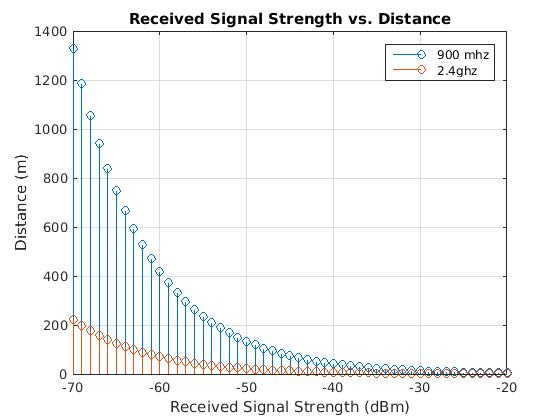
\includegraphics[width=\linewidth]{figures/rss-vs-distance.jpg}
        \caption{\label{fig:log-distance}RSSI readings of NLoS and LoS APs acquired with a stationary agent}
    \end{figure}

    The main motivation behind employing multisource information is to exploit the diversity of the propagation characteristics of the different frequencies.
    As it can be seen in the \Cref{eq:log-distance} and \Cref{fig:log-distance}, the received power and separation distance has a log-linear relationship.
    %  demonstrates the log-distance relationship between received power and the separation between two antennas in two different frequencies in \gls{uhf} radio band.
    This figure implies two fundamental problems in radiolocationing systems:
    The first problem is that as the carrier frequency increases path loss increases significantly, which limits the radio covarage and localization ability of the system in large environments.
    On the other hand, as the carrier frequency increases, the separation between two antennas, i.e.\ the anchor node and the target to be localized, can be identified with finer spatial resolution.
    Therefore, the trade-off between radio coverage and spatial localization resolution can be resolved by employing different frequencies in indoor localization systems by fusing the information acquired from the anchor nodes using different carrier frequency.
    Thus, \gls{mfms} employs a \gls{lora} radio (900 MHz), a WiFi \gls{ap} and a Bluetooth (2.4 GHz) beacon in each anchor nodes.
    \Cref{tab:specs} tabulates the specifications of the radios consisting each anchor node, while \Cref{fig:module} demonstrates the details of the anchor nodes.
    In detail, wider spatial coverage is achieved by using \gls{lora} modules working at 900 MHz while finer spatial resolution provided by WiFi and Bluetooth both working at 2.4 GHz frequency.

    \begin{table}
    \begin{center}
    \caption{\label{tab:specs}The specifications of radios used in anchor nodes}
      \begin{tabular}{@{}lccc@{}}\toprule[1.5pt]
        Property                        &WiFi           &Bluetooth      &\gls{lora}\\ \midrule[1.5pt]
        Frequency [MHz]:                &2400           &2400           &900 \\ \midrule
        Communication Bandwidth:        &1-11 Mbps      &Upto 4 Mbps    &10 Kbps \\ \midrule
        Transmission Power $P_t$ [dBm]: &17             &10             &24 \\ \midrule
        Reciever Sensivity [dBm]:       &?              &-98            &-101 \\ \midrule
        Communication Range [m]:        &$<$20          &$~$10            &$>$100  \\\bottomrule[1.5pt]
      \end{tabular}
    \end{center}
    \end{table}

    \begin{figure}[thpb]
       \centering
       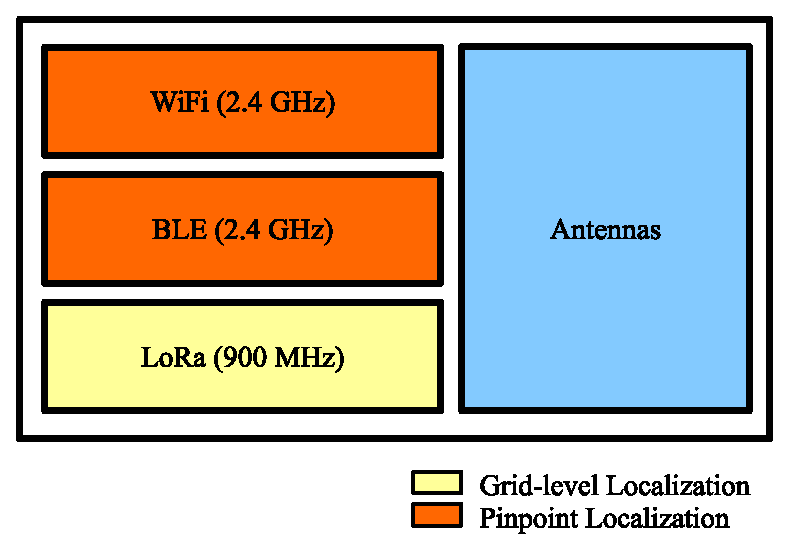
\includegraphics[width=\linewidth]{figures/mfms_module.eps}
       \caption{\label{fig:module}\gls{mfms} Anchor Nodes}
    \end{figure}

    \subsection{Spatially-coherent Path Loss Exponent Estimation}
    This section covers the details of the joint path loss exponent estimation  which forms the first stage of \gls{mfms}.
    We approach the \gls{firl} problem in the scope of curve fitting.
    However, unlike many approaches proposed mentioned earlier, \gls{mfms} does not try to blindly fit a function which best explains the training data given the location labels.
    Moreover, \gls{mfms} does not consider the path loss exponent as a variable describing the whole localization environment.
    Instead, we approach the problem as curve fitting for path loss exponent differing in value depending on the regions in the environment agent resides.
    In detail, the path loss exponent for \gls{mfms} is a function of both location.
    Therefore, the proposed system is able account for non-uniform distribution of obstructions in space.

    \begin{figure}[thpb]
       \centering
       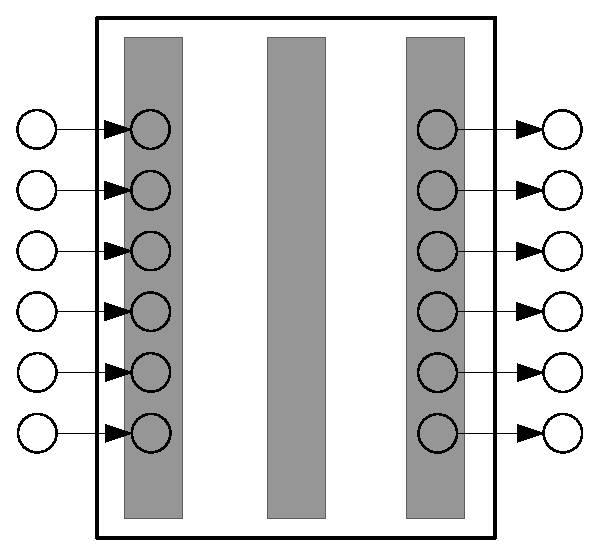
\includegraphics[width=\linewidth]{figures/softmax.eps}
       \caption{\label{fig:softmax}The softmax classifier assigns weights for each anchor node based on the evidence representing the probability of residing in a grid cell $g$.}
    \end{figure}

    Let $\Omega=\{g_i | i=1\ldots n_{grid}\}$, is the localization environment which is divided into $n_{grid}$ number of grids $g$.
    An arbitrary position $\bm{x} \in \Omega$ can be in a shadowed region for any anchor node; thus, \gls{mfms} selectively chooses which anchor nodes to use to localize the agent in $\Omega$.
    This selection is performed by mapping the measurement vector acquired at time step $k$ $\bm{m}^{k}_j \in \mathbb{Z}^{n_{node}}$ with a set of weights $\bm{w}_g \in \mathbb{R}^{n_{node}}$ such that $\sum_g \bm{w}_g = 1$.
    The weights of each grid is learned with a softmax classifier, which is depicted in \Cref{fig:softmax}.
    The classifier is solely based on \gls{lora} measurements due to the fact that the higher probability of observing multiple \gls{lora} modules in arbitrary positions in the environment, thanks to the smallar path loss they introduce.
    \Cref{eq:weighted_m} shows the result of the selection process.

    \begin{equation}
        \label{eq:weighted_m}
        \bm{\widetilde{m}}^{k}_j = \bm{w}_g \bm{m}^{k}_j
    \end{equation}

    For each anchor node, the path loss exponent is estimated with \gls{ldpl} model in a least square sense.
    The estimated spatially-coherent path loss exponent, a set physical parameter defining the radio wave propagation, is incorporated into the location estimation process explained in Stage-II\@.

    \begin{equation}
        n^{*,i}_g = \argmin_n\ \sum_j \left(\norm{\bm{x}_g}_2 - f_d(m^i_{j_g},n)\right)^2
    \end{equation}
    where $\bm{x}_g$ and $m^i_{j_g}$ denote the center position of grid $g$, and measurements acquired in grid $g$, while $f_d(\cdot)$ denotes \gls{ldpl} model.

    \subsection{Pinpoint Localization}
    This section gives details of the second stage of the \gls{mfms} which is the pinpoint localization.
    After localizing the agent in grid-level and selecting which anchor nodes to be employed, the propagation function $\hat{g}_d(\cdot)$ can be formulated as below:
    % , which $\mathbb{Z}^{n_{node}\times n_m} \mapsto \mathbb{R}^2$:
    % Similar to \gls{ldpl}, our radio wave function approximation is given below:
    \begin{equation}
        \label{eq:propfunct}
        \hat{g}_d(\bm{\widetilde{m}}^{k-n_{m}:k}_j, \bm{n}^*_g)= \bm{\hat{x}}
    %   n(k,t)^* = \argmin_n \bm{e}^i  = \argmin_n \{d^i_j - \hat{f}^i_d(m_i, n, t)\}
    \end{equation}
    where $\bm{\widetilde{m}}^{k-n_{m}:k}_j$, $\bm{n}^*_g$, and $\bm{\hat{x}}$ are the weighted measurement vector between time steps $k-n_m$ and $k$, the estimated path loss exponent vector of each anchor node for grid $g$ and the estimated absolute position of the agent, respectively.
    As it can be seen in \Cref{eq:propfunct}, the propagation function incorporates the weighted measurements with the spatially- and temporally-coherent path loss exponent so that the physical characteristics of the radio waves, represented with the path loss, are enforced into the model as a parameter.

    \begin{figure}[thpb]
       \centering
       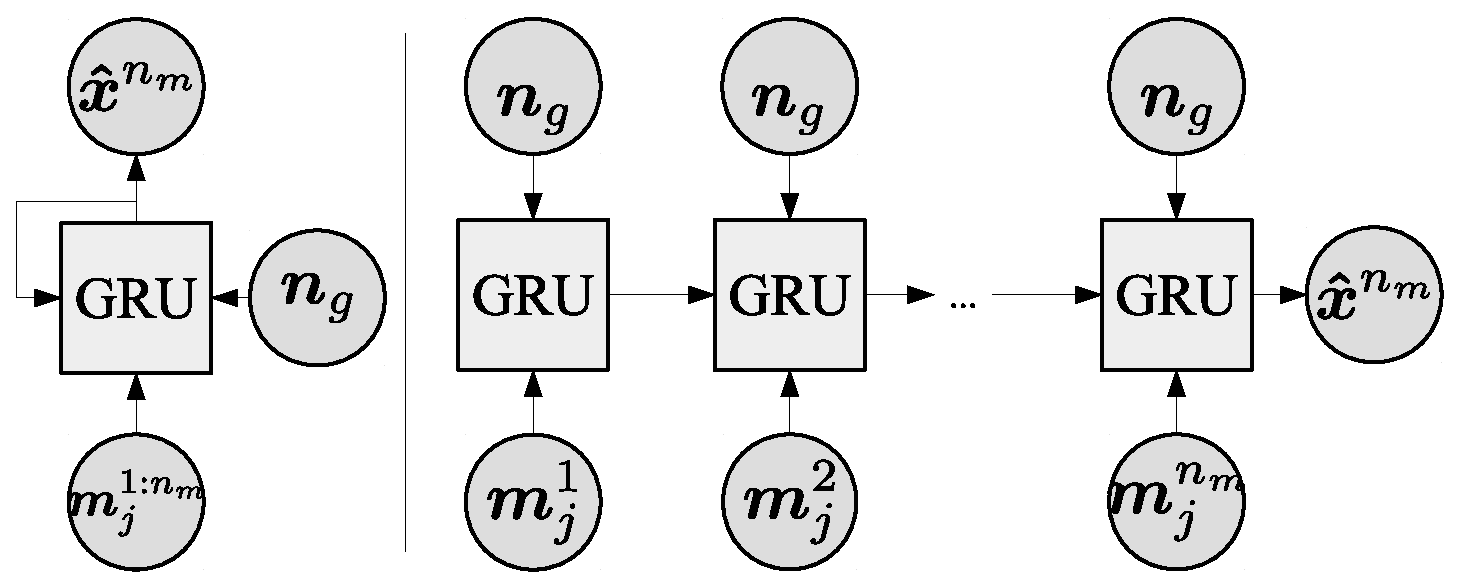
\includegraphics[width=\linewidth]{figures/gru.eps}
       \caption{\label{fig:gru}GRU}
    \end{figure}

    The propagation function of WiFi $\hat{g}^w_d(\cdot)$ and Bluetooth $\hat{g}^b_d(\cdot)$ anchors are approximated with two separate recurrent neural networks, consisting of three layers of \gls{gru}~\cite{cho2014learning}.
    These functions are attained with a \gls{sgd} based back-propagation algorithm.
    After approximating the propagation functions, these are employed to estimate the location of the agent.
    Specifically, the pinpointing algorithm incorporates the spatially-coherent path loss exponent along with the weighted measurements to estimate $\bm{\hat{x}}^w$ and $\bm{\hat{x}}^b$, estimated positions by using WiFi measurements and Bluetooth measurements, respectively.

    \Cref{fig:gru} depicts the Stage-II of \gls{mfms} in an unfolded representation.
    % The locatization environment is divided into $n_{grid}$ number of grids in order to obtain


    \subsection{Information Fusion}
    This section of the paper further explains the Stage-III of the \gls{mfms}.
    The Stage-III is essentially an information fusion layer of the model where location estimates of WiFi and Bluetooth measurements are fused into one final entity.
    The incorporation of two estimates are achieved in the framework of a \gls{nn} consisting of 3 layers.
    The network is in a gradually narrowing structure such that the first, second and last layer contain 8, 4, 2 neurons, respectively.
    \Cref{fig:fusion} demonstrates the Phase-III\@.

    \begin{figure}[thpb]
       \centering
       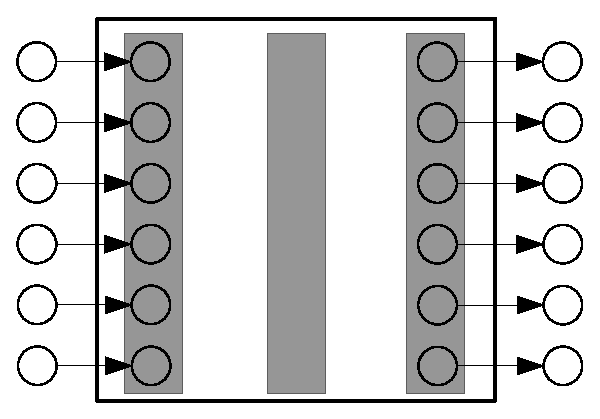
\includegraphics[width=0.95\linewidth]{figures/fusion.eps}
       \caption{\label{fig:fusion}Two location estimates of WiFi and Bluetooth approximations are fused with a 3 layered-\gls{nn}.}
    \end{figure}


\section{Experimentation}

    \subsection{Experimental Setup}
    Lorem ipsum dolor sit amet, consectetur adipisicing elit, sed do eiusmod tempor incididunt ut labore et dolore magna aliqua. Ut enim ad minim veniam, quis nostrud exercitation ullamco laboris nisi ut aliquip ex ea commodo consequat. Duis aute irure dolor in reprehenderit in voluptate velit esse cillum dolore eu fugiat nulla pariatur. Excepteur sint occaecat cupidatat non proident, sunt in culpa qui officia deserunt mollit anim id est laborum.
    \subsubsection{Hardware}
    Lorem ipsum dolor sit amet, consectetur adipisicing elit, sed do eiusmod tempor incididunt ut labore et dolore magna aliqua. Ut enim ad minim veniam, quis nostrud exercitation ullamco laboris nisi ut aliquip ex ea commodo consequat. Duis aute irure dolor in reprehenderit in voluptate velit esse cillum dolore eu fugiat nulla pariatur. Excepteur sint occaecat cupidatat non proident, sunt in culpa qui officia deserunt mollit anim id est laborum.
    \subsubsection{Software}
    Lorem ipsum dolor sit amet, consectetur adipisicing elit, sed do eiusmod tempor incididunt ut labore et dolore magna aliqua. Ut enim ad minim veniam, quis nostrud exercitation ullamco laboris nisi ut aliquip ex ea commodo consequat. Duis aute irure dolor in reprehenderit in voluptate velit esse cillum dolore eu fugiat nulla pariatur. Excepteur sint occaecat cupidatat non proident, sunt in culpa qui officia deserunt mollit anim id est laborum.
    Lorem ipsum dolor sit amet, consectetur adipisicing elit, sed do eiusmod tempor incididunt ut labore et dolore magna aliqua. Ut enim ad minim veniam, quis nostrud exercitation ullamco laboris nisi ut aliquip ex ea commodo consequat. Duis aute irure dolor in reprehenderit in voluptate velit esse cillum dolore eu fugiat nulla pariatur. Excepteur sint occaecat cupidatat non proident, sunt in culpa qui officia deserunt mollit anim id est laborum.
    ROS~\cite{quigley2009ros}
    Keras~\cite{chollet2015}
    Tensorflow~\cite{tensorflow2015-whitepaper}
    \subsection{Results}
    Lorem ipsum dolor sit amet, consectetur adipisicing elit, sed do eiusmod tempor incididunt ut labore et dolore magna aliqua. Ut enim ad minim veniam, quis nostrud exercitation ullamco laboris nisi ut aliquip ex ea commodo consequat. Duis aute irure dolor in reprehenderit in voluptate velit esse cillum dolore eu fugiat nulla pariatur. Excepteur sint occaecat cupidatat non proident, sunt in culpa qui officia deserunt mollit anim id est laborum.

    \begin{figure}[thpb]
        \centering
        
\includegraphics[width=\linewidth]{figures/placeholder.png}
        \caption{\label{fig:confussion}The confusion matrix obtained during grid-selection.}
    \end{figure}

    Lorem ipsum dolor sit amet, consectetur adipisicing elit, sed do eiusmod tempor incididunt ut labore et dolore magna aliqua. Ut enim ad minim veniam, quis nostrud exercitation ullamco laboris nisi ut aliquip ex ea commodo consequat. Duis aute irure dolor in reprehenderit in voluptate velit esse cillum dolore eu fugiat nulla pariatur. Excepteur sint occaecat cupidatat non proident, sunt in culpa qui officia deserunt mollit anim id est laborum.
    Lorem ipsum dolor sit amet, consectetur adipisicing elit, sed do eiusmod tempor incididunt ut labore et dolore magna aliqua. Ut enim ad minim veniam, quis nostrud exercitation ullamco laboris nisi ut aliquip ex ea commodo consequat. Duis aute irure dolor in reprehenderit in voluptate velit esse cillum dolore eu fugiat nulla pariatur. Excepteur sint occaecat cupidatat non proident, sunt in culpa qui officia deserunt mollit anim id est laborum.

    \begin{figure}[thpb]
        \centering
        
\includegraphics[width=\linewidth]{figures/placeholder.png}
        \caption{\label{fig:cdf}Cumulative Distribution Function of the Localization Error in both environment: The red, blue and green lines depict localization error occurred when WiFi, Bluetooth and fused measurements are used in localization, respectively.}
    \end{figure}
    Lorem ipsum dolor sit amet, consectetur adipisicing elit, sed do eiusmod tempor incididunt ut labore et dolore magna aliqua. Ut enim ad minim veniam, quis nostrud exercitation ullamco laboris nisi ut aliquip ex ea commodo consequat. Duis aute irure dolor in reprehenderit in voluptate velit esse cillum dolore eu fugiat nulla pariatur. Excepteur sint occaecat cupidatat non proident, sunt in culpa qui officia deserunt mollit anim id est laborum.
    Lorem ipsum dolor sit amet, consectetur adipisicing elit, sed do eiusmod tempor incididunt ut labore et dolore magna aliqua. Ut enim ad minim veniam, quis nostrud exercitation ullamco laboris nisi ut aliquip ex ea commodo consequat. Duis aute irure dolor in reprehenderit in voluptate velit esse cillum dolore eu fugiat nulla pariatur. Excepteur sint occaecat cupidatat non proident, sunt in culpa qui officia deserunt mollit anim id est laborum.


\begin{figure*}[!ptbhp]
  \centering
  \begin{subfigure}[t]{0.45\linewidth}
    
\includegraphics[width=\columnwidth]{figures/placeholder.png}
    \caption{Floor map of the first environment used in the experimentations}\label{fig:randolph}
  \end{subfigure}
  \begin{subfigure}[t]{0.45\linewidth}
    
\includegraphics[width=\columnwidth]{figures/placeholder.png}
    \caption{Floor map of the first environment used in the }\label{fig:goodwin}
  \end{subfigure}
  \caption{The floor maps of the environments was conducted\label{fig:environment}}
\end{figure*}


\section{Conclusions and Future Work}
\label{sec:conclusion}
\begin{enumerate}
    \item P-1: Summary: Copy and paste from ``this paper presents'', paraphrase it, while summarizing it.
    \item P-2: Results and Conclusions: Copy preface of numerical results section. For each results, add a resulting remark. Then conclude with a statement: ``Results have demonstrated the effectiveness and applicability of the proposed approach.''
    \item P-3: Future work: This paper has focused on \ldots and much work is still left open; describe a few future works.
\end{enumerate}
Lorem ipsum dolor sit amet, consectetur adipisicing elit, sed do eiusmod tempor incididunt ut labore et dolore magna aliqua. Ut enim ad minim veniam, quis nostrud exercitation ullamco laboris nisi ut aliquip ex ea commodo consequat. Duis aute irure dolor in reprehenderit in voluptate velit esse cillum dolore eu fugiat nulla pariatur. Excepteur sint occaecat cupidatat non proident, sunt in culpa qui officia deserunt mollit anim id est laborum.
Lorem ipsum dolor sit amet, consectetur adipisicing elit, sed do eiusmod tempor incididunt ut labore et dolore magna aliqua. Ut enim ad minim veniam, quis nostrud exercitation ullamco laboris nisi ut aliquip ex ea commodo consequat. Duis aute irure dolor in reprehenderit in voluptate velit esse cillum dolore eu fugiat nulla pariatur. Excepteur sint occaecat cupidatat non proident, sunt in culpa qui officia deserunt mollit anim id est laborum.

Lorem ipsum dolor sit amet, consectetur adipisicing elit, sed do eiusmod tempor incididunt ut labore et dolore magna aliqua. Ut enim ad minim veniam, quis nostrud exercitation ullamco laboris nisi ut aliquip ex ea commodo consequat. Duis aute irure dolor in reprehenderit in voluptate velit esse cillum dolore eu fugiat nulla pariatur. Excepteur sint occaecat cupidatat non proident, sunt in culpa qui officia deserunt mollit anim id est laborum.
Lorem ipsum dolor sit amet, consectetur adipisicing elit, sed do eiusmod tempor incididunt ut labore et dolore magna aliqua. Ut enim ad minim veniam, quis nostrud exercitation ullamco laboris nisi ut aliquip ex ea commodo consequat. Duis aute irure dolor in reprehenderit in voluptate velit esse cillum dolore eu fugiat nulla pariatur. Excepteur sint occaecat cupidatat non proident, sunt in culpa qui officia deserunt mollit anim id est laborum.

Lorem ipsum dolor sit amet, consectetur adipisicing elit, sed do eiusmod tempor incididunt ut labore et dolore magna aliqua. Ut enim ad minim veniam, quis nostrud exercitation ullamco laboris nisi ut aliquip ex ea commodo consequat. Duis aute irure dolor in reprehenderit in voluptate velit esse cillum dolore eu fugiat nulla pariatur. Excepteur sint occaecat cupidatat non proident, sunt in culpa qui officia deserunt mollit anim id est laborum.
Lorem ipsum dolor sit amet, consectetur adipisicing elit, sed do eiusmod tempor incididunt ut labore et dolore magna aliqua. Ut enim ad minim veniam, quis nostrud exercitation ullamco laboris nisi ut aliquip ex ea commodo consequat. Duis aute irure dolor in reprehenderit in voluptate velit esse cillum dolore eu fugiat nulla pariatur. Excepteur sint occaecat cupidatat non proident, sunt in culpa qui officia deserunt mollit anim id est laborum.


\section*{ACKNOWLEDGMENT}
Turkish Government and stuff


\bibliographystyle{IEEEtran}
\bibliography{bibliography}

\end{document}
